 \section*{Решения и комментарии}

\subsubsection*{Определение большинства}% (IDENTIFYING THE MAJORITY)

Идея состоит в том, что каждый раз, когда на счётчике появляется 0 (начальная позиция), 
вы запоминаете имя, которое слышите в данный момент, и добавляете на счётчике 1.
Когда на счётчике больше, чем 0, вы прибавляете, если имя, которое вы слышите то же, что вы держите в уме.
В противном случае отнимаете на счётчике 1, но сохраняете в уме прежнее имя.

Возможно, конечно, закончить с именем, которое называлось только один раз (например, если список был «Aлиса, Боб, Алиса, Боб, Алиса, Боб, Чарли»).
Тем не менее, если имя появлялось больше, чем половина раз, то оно гарантированно сохранится у вас в уме до конца.
Причина того, что имя останется в вашей памяти, состоит в том, что на счётчике больше прибавляется, чем отнимается.

Данный алгоритм описан в статье Майкла Фишера и Стивена Зальцберга.\footnote{M. J. Fischer and S. L. Salzberg, \emph{Finding a Majority Among n Votes} Journal of Algorithms Vol. 3, No 4 (December 1989), pp 362--380}

\subsubsection*{Обездвиживатель конвея}% (THE CONWAY IMMOBILIZER)

Непросто придумать алгоритм, который успешно продвигается вперёд, избегает зацикливания и не делает никаких глупостей, когда вы уже практически дошли до цели.
В данной задаче сработает следующий трюк.

Перекладываете карту направо (по кругу, если понадобится) на пустую колоду, если такая имеется, кроме случаев К, --- , Т или К, Т, --- , при которых нужно положить туза на короля.
Если открыты все карты и дама находится в левой колоде, кладёте на даму короля, в противном случае, карту справа от дамы перекладываете на одну колоду вправо (опять же, можно при необходимости двигаться по кругу).
Очевидно, что нет хода, который собирает три карты в стопку, если только изначально не была выигрышная комбинация.
Комбинация два --- один, даже такая, как К, --- , Т или
К, Т, --- , откроет все карты максимально за три хода (если игра еще не выиграна).
Таким образом, достаточно проверить (смотрите прилагаемую диаграмму), что все шесть возможных комбинаций открытых карт приводят к победе.
\heart

Удивительным образом, этот алгоритм можно обобщить для работы с любым количеством карт (фиксированным, известным), оперируя всё теми же тремя колодами.
Скажем, для 52 карт, пронумерованных от 1 до 52, следующие правила (данные в приоритетном порядке) в конечном итоге приведут к тому, что слева окажется колода, сложенная по-порядку с 1 наверху.

Итак, если вы видите:

\begin{enumerate}[(1)]
\item $2, 1, -$, то кладёте $1$ на $2$;
\item две произвольные карты, --- перекладываете карту направо (по кругу, если необходимо) на пустую колоду;
\item $k, j, k-1,$ где $j < k$, --- кладёте $k-1$ на $k$;
\item только одну карту, --- перекладываете карту налево;
\item три карты, --- карту справа от наибольшей перекладываете направо.
\end{enumerate}

\begin{figure}[h!]
\centering
\includegraphics[scale=0.55]{Figs/Handicaps/conway}
\end{figure}

Докажем, что этот алгоритм действительно работает.
Предположим, что карта 52 открыта и лежит на средней или на правой колоде.
Тогда, следуя правилу (2) и (5), она в итоге окажется в левой колоде вместе со всеми остальными картами из средней колоды.
По мере их перемещения вправо согласно правилу (2), карты $51, 50, 49, \dots, k$ будут складываться на 52 согласно правилу (3) для некоторых $k < 52$, и средняя колода опустеет.
Разумеется, если $k = 1$, мы решили задачу, правило (1) сделало последний ход.
В противном случае карта $k$ переместится в среднюю колоду по правилу (2) и в правую по правилу (5), за ней аналогичным образом последует карта $k+1$, и так далее, пока в правой колоде не окажется 51 карта, сложенные по-порядку, с картой 51 внизу и картой $k$ наверху.

Теперь карта 52 кладётся на среднюю колоду, а правая колода перекладывается в обратном порядке на левую колоду, карта 52 передвигается на правую колоду, левая колода перемещается на среднюю колоду, снова меняя порядок, и карта 52 перекладывается обратно на левую колоду.
В этот момент в средней колоде окажутся карты от 51 до $k$, с 51 наверху.
Дальше карты с 51 до $k$ перемещаются согласно правилу (2) направо и оказываются в левой колоде по правилу (3), до тех пор пока, опять, $k, k+1, \dots, 52$ не попадут в левую колоду.

Правая колода сейчас пустая, следовательно, карта $k-1$ находится где-то в средней колоде.
Если она не в самом низу, она перейдёт в левую колоду и процесс, описанный выше, повторится для $k' < k$.
Если случилось так, что она оказалась в самом низу колоды, она не попадёт влево (если только, это не карта 1), потому что, когда она переместится вправо по правилу (5), средняя колода окажется пустой, и мы вынуждены применить правило (2) вместо (3).
Однако, в конце следующего цикла, в средней колоде будет обратный порядок, с картой $k-1$ наверху.
Отсюда следует, что хотя бы каждый второй раз, когда карта 52 снова кладётся на пустую левую колоду, порядок $k$ уменьшается.

Мы сможем завершить доказательство, если покажем, что предполагаемое выше условие, что карта 52 находится на верху средней или правой колоды, должно когда-нибудь случиться.
Предположим вначале, что карта 52 лежит на верху левой колоды (все остальные карты под ней).
Тогда она может собрать карты $51, 50, \dots, k$ над собой, следуя правилу (3), а остальные карты окажутся в средней и, возможно, в правой колоде.
Затем правила (2) и (5) опустошат среднюю колоду.
Карта $k$ переместится в середину и потом вправо, затем, аналогично, карта $k+1$, и так далее (как и выше), пока карта 52 снова не окажется наверху, но на этот раз (после того, как карта 51 перешла на правую колоду) средняя колода будет пустая.
Карта 52 кладётся тогда на среднюю колоду, и мы получаем желаемое условие.

\subsubsection*{Крутящиеся выключатели}% (SPINNING SWITCHERS)

Эта задача попала ко мне от Саши Барга из Мэрилендского университета, но, похоже, она была уже довольно известна.
Как и во многих задачах, здесь будет полезно рассмотреть вначале более простую версию.
Возьмём вариант с двумя выключателями: нажав на обе кнопки, мы выясним, находились ли они в одинаковом состоянии, если да, то лампочка загорится (если она уже не горела).
В противном случае, на следующем шаге нажмём одну кнопку, после этого кнопки \emph{будут} в одинаковом состоянии, и в наихудшем случае нам придётся сделать ещё один шаг, нажав обе кнопки, чтобы лампочка зажглась.

Вернёмся к варианту с четырьмя лампочками.
Обозначим через 
А операцию, когда мы нажимаем все четыре кнопки, 
D --- диагональные кнопки, 
N --- соседние и 
S --- одну кнопку.
Тогда последовательность операций ADANASADAND включит лампочку не более, чем за 12 шагов.

В более общем виде для выключателей в углах $n=2^k$-угольника это можно сделать за $2^n-1$ шаг следующим образом.
Пусть $X=X_1,\dots,X_m$ шаги для $\tfrac n2=2^{k-1}$-угольника.
Составим из противоположных выключателей пары, если $X_i$ --- шаг для $\tfrac n2$-угольника, при котором нажимаются кнопки $i_1,\dots,i_j$, тогда пусть $X_i'$ будет шагом для $n$-угольника, при котором нажимаются кнопки $i_1,\dots,i_j$ и $i_1+\tfrac n2,\dots,i_j+\tfrac n2$.
Пусть $X'$ обозначает последовательность шагов $X_1',\dots,X_m'$.

Нам также необходим шаг $X_i''$ для $n$-угольника, при котором нажимаются только кнопки $i_1,\dots,i_j$.

Будем говорить про противополжную пару, что она «чётная», если оба выключателя включены или выключены.
Если все пары чётные, тогда применение шага $X'$ включит все выключатели.
Идея в том, чтобы посредством применения шаги $X_1'',X_2''$ и так далее, сделать все пары чётными, каждый раз проверяя при помощи $X'$, добились ли мы успеха.
Порядок шагов такой:
\begin{align*}
X_1',\dots,X_m';X_1'';X_1',\dots,X_m';X_2'';
\\
X_1',\dots,X_m';\dots,:X_m'';X_1',\dots,X_m',
\end{align*}
или, более компактно: $X';X_1'';X',X_2'';X';\dots,X_m'',X'$.
Всего получилось $(m+1)m+m=m(m+2)$ шагов.
Следовательно, если $f(n)$ число шагов, предпринятых для решения $n$-угольника, то $f(2n)=(2^n-1)(2^n+1)=2^{2n}-1$ и $f(1)=2^1-1=1$, итак, это проверено.

Эта последовательность действий работает, потому что шаги типа $X''$ работают на чётных/нечётных парах также, как и шаги типа $X$ работали на включенных/выключенных парах, и, между тем, шаги типа $X'$ абсолютно не влияют на конфигурацию чётных/нечётных пар.
\heart

С другой стороны, задача не разрешима, если $n$ не является степенью двойки, например, если $n=m2^k$, при нечётном $m$.
Для представления одновременно конфигурации выключателей (1 = «включен», 0 = «выключен») и операции (1 = «нажать», 0 = «не трогать») можно прибегнуть к бинарным векторам длины .
Пусть $v$ такой вектор, и пусть $v^i$ обозначает результат его поворота на $i$ шагов вправо.
Применение операции $w$ к конфигурации $v$ приведёт к конфигурации $v+w$, если поворота не было, но так как он имеется, мы получаем $v+w^i$ для некоторого значения $i$.

Будем говорить, что $n$-вектор $v$ является «неровным», % [rough ?], 
если число различных его вращений $v^0,v^1,\dots,v^{n-1}$ не равно степени двойки.
Предположим (как и в начале), что любая неровная конфигурация возможна при некотором вращении.
Далее мы утверждаем, что после любой фиксированной операции $w$ любая неровная конфигурация все ещё возможна при некоторых вращениях.
Таким образом нет гарантированного способа избавится от неровных конфигураций и, в частности, нельзя гарантировать получения $11\dots1$.

Для нечётного $n$, то есть если $n=m$, все векторы, кроме $00\dots0$ и $11\dots1$ неровные.
Если $w$ некий вектор и $v$ неровный вектор, то $v-w$ (то же что и $v+w$), или $v-w^1$ будут неровными, так что, если у одного из векторов до применения операции было вращение, то вращение теперь должно быть у вектора???

Если $n=m2^k$, при $k>1$, то можно разбить $n$-цикл на сегменты длины $2^k$ и $u$ будет неровным до тех пор, пока он не одинаковый на всех сегментах.
Следовательно, если он неровный, то существует $1\le j\le 2^k$, что координаты $i2^k+j$ для $1\le j\le m$ не все равны.
И теперь, можно применить рассуждение выше, рассматривая только эти координаты.

\subsubsection*{Комната с одной лампочкой}% (THE ONE-BULB ROOM)

Я услышал эту задачу от Адама Чэлкрафта (Adam Chalcraft), который имеет честь представлять Великобританию на международных соревнованиях по одноколёсному хоккею.
Задача также появлялась на сайте www.ibm.com и была перепечатана в Emissary, информационном бюллетене Математического института в Беркли. %(Matematical Science Research Institute) 
Одна из версий задачи появлялась даже в заслуженно известной программе Национального Общественного радио «Car Talk» в 2003 году.

Однако, считаю нужным предупредить читателя, что эту задачу иногда путают с куда более сложной задачей, с которой вам предстоит встретиться в следующей главе.

\medskip

Безусловно, необходимо предположить, что между посещениями заключённых никто в комнате лампочкой не балуется.
Заключённым необязательно знать, в каком состоянии изначально находится лампочка.
Идея заключается в том, что один из заключённых (скажем, Алиса) всё время пытается лампочку включить, а каждый из остальных выключает её два раза.

То есть, более подробно, Алиса всегда включает лампочку, если она выключена, в противном случае, оставляет её включённой.
Остальные заключённые выключают её первые два раза, если она включена, и оставляют её гореть при последующих посещениях.

Алиса считает, сколько раз она попадает в тёмную комнату после своего первого 
посещения, после $2n-3$ тёмных визитов, она может заключить, что все побывали в комнате.
Почему?
Каждое тёмное посещение говорит о том, что один из остальных $n-1$ заключённых побывал в комнате.
Если же кто-то из них, скажем, Боб, не посещал комнаты, тогда лампочка не могла быть выключена больше, чем $2(n-2)=2n-4$ раз.
С другой стороны, Алиса в конце концов должна будет достичь её $2n-3$ тёмных визитов, потому что в итоге лампочка будет выключена $2(n-1)=2n-2$
раз и только одно из этих выключений (если один из заключённых побывал в комнате до первого визита Алисы и выключил изначально горящую лампочку) может не засчитаться Алисой за тёмный визит.

Если заключённых только два, ясно, что каждый из них узнаёт о том, побывал ли другой в комнате, поскольку Алиса дожидается её первого тёмного повторного посещения, в то время как Боб ждёт свой первый \emph{светлый} повторный визит.
Однако, для $n>2$ заключённых имеется доказательство того, что невозможно гарантировать, что больше, чем один заключённый сможет сказать, посетили ли все остальные комнату.
Ниже приводится набросок доказательства.
Читателям рекомендуется его пропустить, если только они специально не заинтересованы в том, как получаются отрицательные результаты в (communications) задачах подобного сорта.
Я включил это доказательство потому, что, насколько мне известно, оно нигде не появлялось.

В основном, мы утверждаем, что противник (который, предполагается, 
знает стратегию заключённых, составляя расписание посещений) может вынуждать их совершать бесполезные действия, отличающиеся от тех, что применялись в протоколе выше.

Давайте сосредоточимся на одном заключённом, Алисе.
Предположим, что её стратегия детерминистическая и основана исключительно на последовательности состояний лампочки, которые она до сих пор наблюдала.

Положим, что стратегия Алисы заставляет её (в некоторых обстоятельствах) изменить состояние (лампочки), после того, как она нашла её в том же состоянии,что и во время своего последнего посещения.
Тогда противник может немедленно отправить её обратно в комнату, «сводя на нет» её предыдущий визит.
В результате, эта часть стратегии Алисы может только дать противнику дополнительную опцию.
Исходя из этого, можно предположить, что Алиса не должна менять состояние лампочки, если она находит её в том же виде, что и в свой последний визит.

Далее, предположим, что Алисе в некий момент требуется оставить лампочку в том же состоянии, в котором она её нашла.
Тогда мы утверждаем, что можно предположить, что после этого она никогда снова не предпримет каких-либо действий! Почему? Потому что, если противник не хочет, чтобы она продолжала действовать, он может устроить так, что Алиса никогда не увидит лампочку в состоянии, отличном от того, которое она видит в данный момент.
Он может это сделать, поскольку, если Алиса действительно останется навсегда неактивной, то, по крайней мере, одно из состояний («включено» или «выключено») будет повторяться бесконечно часто.
Положим, это «выключено».
Тогда противник может составить расписание для Алисы так, что лампочка будет выключена как в её посещении сейчас, так и во всех последующих, и следовательно, согласно предыдущему рассуждению, она никогда не будет снова действовать.
Итак, eщё раз, у противника всегда есть возможность заставить Алису замолчать, и можно предположить, что это его единственная возможность.

Очевидно, Алиса не может начинать с инструкции оставить лампочку в том же состоянии, как она её находит, так как в этом случае она перестанет действовать совсем, и никто никогда не узнает, посещала ли она комнату.%
\footnote{Если только она не пользуется очень сильными духами...}
Скажем, она должна включить лампочку, если она выключена, в обратном случае оставить лампочку как есть.
Тогда она ничего не будет делать до тех пор, пока опять не попадёт в комнату с выключенной лампочкой, и в этом случае она может только снова включить лампочку или остаться бездейственной навсегда.
Таким образом, число раз, когда Алиса включает лампочку, ограничено $j$ (которое может быть константой, иначе у противника будет больше преимуществ).
Назовём эту стратегию $+j$, где $j$ положительное целое число или бесконечность.
Аналогичное рассуждение, применённое для случая, когда Алиса должна во время первого визита выключить лампочку, приводит к стратегии $-j$.

Остаётся только один возможный вариант, когда Алиса должна будет изменить состояние лампочки в свой первый визит в комнату, но в этом случае далее она вынуждена будет продолжить действовать так, как описано выше, в зависимости от того, включила она лампочку или выключила.
И это снова даёт противнику дополнительное преимущество.

Это сводится к тому, что у каждого заключённого имеется стратегия $+j$ или $-j$ для различных $j$.
Если все они только выключают (или включают) лампочку, никто ничего не сможет определить.
Таким образом, можно предположить, что у Алисы стратегия $+j$, а у Боба $-j$.
Если Чарли включает лампочку, Алиса никогда не сможет определить, был ли это последний визит Боба или Чарли, и у Боба и Чарли остаётся ещё по одному заданию.
Если Чарли выключает лампочку, то тогда Боб --- это тот, кому достанется «тёмный визит».

Учитывая всё вышесказанное, мы получаем, что для того, чтобы какой-то заключённый смог определить, что все посетили комнату, Алиса должна включить лампочку, в то время как все остальные её выключают (или наоборот).
Действительно, если у Алисы стратегия $+j_1$, а у других  $-j_2,\dots,-j_n$ стратегии тогда легко проверить, что условие, при котором каждое $j_i$ конечно и не меньше 2, а $j_1$ больше, чем сумма остальных минус наименьший из них, является необходимым и достаточным.

Отсюда следует, что если $n>2$, тогда максимум одному заключённому гарантирована честь знать, все ли побывали в комнате.
Уфф!

\subsubsection*{Два шерифа}% (ТHE TWO SHERIFFS)

Если два шерифа (назовём их Лев и Ральф) обмениваются секретной информацией, они могут использовать этот секрет для того, чтобы зашифровать свой разговор и достичь цели.
Но так как они никогда прежде не встречались, им нужно будет, на самом деле, изготовить этот свой собственный секрет.

\medskip

Будем всегда предполагать, что пары, к которым Лев и Ральф сузили свои списки подозреваемых, не одинаковы, то есть существует возможность определить убийцу.
Заметим, что, если, скажем, Лев просто называет свою пару, тогда Ральф будет знать, кто убийца.
Но тогда и банда линчевателей будет знать всё, что знает Лев, так что любая попытка Ральфа сообщить Льву имя убийцы, без того, чтобы об этом не прознали линчеватели, обречена на провал.

Очевидно, Лев и Ральф должны подойти к определению имени убийцы более хитрым способом.
Составим таблицу из всех возможных пар подозреваемых таким образом, что каждый столбец содержит разбиение восьми подозреваемых на четыре пары.
Вот один из способов:

\[
\begin{matrix}
\{1,2\}&\{1,3\}&\{1,4\}&\{1,5\}&\{1,6\}&\{1,7\}&\{1,8\}
\\
\{3,4\}&\{2,4\}&\{2,3\}&\{2,6\}&\{2,5\}&\{2,8\}&\{2,7\}
\\
\{5,6\}&\{5,7\}&\{5,8\}&\{3,7\}&\{3,8\}&\{3,5\}&\{3,6\}
\\
\{7,8\}&\{6,8\}&\{6,7\}&\{4,8\}&\{4,7\}&\{4,6\}&\{4,5\}
\end{matrix}
\]


Лев и Ральф совершенно свободно могут обсуждать по телефону вопрос о сокрытии информации от линчевателей.
В частности, ничто не может помешать им согласиться пронумеровать подозреваемых и составить такую таблицу, как приведённая выше.

Дальше Лев сообщает Ральфу, в каком столбце находится его пара.
Например, если пара Льва $\{1,2\}$, он говорит: «Моя пара в первом столбце.» 

Если пара Ральфа находится в том же столбце, он тут же понимает, что у него и Льва одинаковые пары.
Он может прямо сказать об этом, после чего шерифам остаётся только повесить трубки и и вернуться к сыскной работе.

В другом случае Ральф понимает, что пара Льва одна из двух пар в столбце.
Вернёмся к нашему примеру, если пара Ральфа $\{2,3\}$, он знает, что у Льва должна быть пара $\{1,2\}$ или $\{3,4\}$.
Затем он разделяет столбец на две равные части, так, чтобы обе предполагаемые пары были в одной части, и сообщает об этом разбиении Льву.

В нашем примере он должен будет сказать Льву: «Моя пара либо в $\{1,2,3,4\}$, либо в $\{5,6,7,8\}$.» (Если же пара Ральфа была бы $\{2,5\}$, он сказал бы: «Моя пара либо в $\{1,2,4,5\}$, либо в $\{3,4,7,8\}$.» )

Лев, безусловно, будет знать, в какой части надо искать пару Ральфа, так как она может быть только в той части, где находится его собственная пара.
Это теперь тайна Ральфа и Льва!

Теперь Лев может сказать Ральфу стоит ли его пара на первом или втором месте в соответствующей части.
Если, как в примере выше, пары $\{1,2\}$ и $\{2,3\}$, Лев может сказать: «Моя пара первая.», или, тоже самое, «Моя пара либо $\{1,2\}$, либо $\{5,6\}$.»

Далее, Ральфу становится ясно, какая пара у Льва, а, следовательно, и кто является убийцей.
Он может сообщить об этом Льву, просто сказав, что убийце в соответствует большее или меньшее число в паре Льва.
То есть, он сказал бы: «Убийца --- самый старший в твоей паре.» , или же: «Убийца --- 2 или 6.»

Банда линчевателей не сможет понять, о какой из «частей» говорят Лев и Ральф.
Если бы у Льва была пара $\{5,6\}$, а у Ральфа $\{6,7\}$ или $\{6,8\}$, то весь разговор, подслушанный линчевателями, был бы абсолютно таким же, как в рассмотренном примере, и в этом случае убийцей оказался бы номер 6 вместо 2.
\heart

Задача о двух шерифах впервые появилась в статье Дональда Бивера, Стюарта Хабера и Питера Винклера.\footnote{D.
Beaver, S. Haber, and P. Winkler On the Isolation of a Common Secret, from The Mathematics of Paul Erd\H{o}s Vol. II, R. L. Gracham and J.Nesetril, editors, Springer-Verlag, Berlin, 1996} Задача была придумана как пример открытия, сделанного вашим автором лет двадцать пять тому назад: а именно --- по открытым каналам связи из общеизвестной информации можно сделать общую тайну.
Первоначально эта идея применялась для игры в Бридж, где партнёрам не разрешается иметь предварительные договорённости о значениях заявок и игре.
С 1924 года, когда был создан современный Бридж, считалось (неверно), что это правило препятствует какому-либо секретному общению между партнёрами.
Это заблуждение оказало весьма сдерживающий эффект на развитие более совершенных методов торговли и стратегии вистующих, так как многие считали, что такие методы могут давать противникам слишком много информации.
Например, основанная на научных методах шлемовая торговля подскажет противнику, как вести игру.

Однако карты у вас в руке (которые, как вы знаете, не должны находиться у вашего партнера) дают вам и вашему партнёру некое общее знание, которое может быть использовано для секретного общения.\footnote{
Подробную информацию и ссылки можно найти в P. Winkler The Advent of Cryptology in the Game of Bridge, Cryptologia Vol.7 \#4 (October 1983), pp 327--332.}

\subsubsection*{Рассеянный профессор}% (THE ABSENT-MINDED PILL TAKER)

Профессорская коробочка для таблеток состоит из семи прозрачных ячеек, помеченных \textsc{вс}, \textsc{пн}, \textsc{вт}, \textsc{ср}, \textsc{чт}, \textsc{пт}, \textsc{сб} (см. рисунок ниже).
Представим, что профессор получает 30 новых таблеток в пятницу утром.
Он хочет распределить их по ячейкам таким образом, чтобы посмотрев на свою коробочку, начиная с этого дня, он мог бы сказать, выпил он свою ежедневную таблетку, и, если нет, мог бы взять её из соответствующей ячейки.

Очевидный способ это сделать --- положить по 5 таблеток в \textsc{пт} и \textsc{сб} и по 4 таблетки в \textsc{вс}, \textsc{пн}, \textsc{вт}, \textsc{ср}, \textsc{чт} и следовать такому алгоритму:
\begin{itemize}
 \item[] Когда коробочка для таблеток содержит непрерывную по модулю 7 строку ячеек с $k$ таблетками, а остаток только с $k-1$, он знает, что самая левая «тяжёлая» ячейка (с $k$ таблетками) --- это то, откуда нужно взять следующую таблетку.
Если это среда, и такая ячейка помечена \textsc{ср}, он берёт оттуда таблетку, если же эта ячейка \textsc{чт}, он знает, что таблетка уже принята.
\end{itemize}

Трудность заключается в том, что каждые семь дней все ячейки становятся равными, то есть, в каждой из них одно и тоже число таблеток.
Какую ячейку нужно тогда выбрать?
Ну, в данном случае, профессор понимает, что это случится в воскресенье, так что он устанавливает правило: когда ячейки равны, \textsc{вс} --- контрольный контейнер.
То есть, если он видит равные ячейки и этот день --- воскресенье, он берёт таблетку из \textsc{вс}, если же это суббота, значит, он уже таблетку принял.

Всё идёт прекрасно до тех пор, пока, 30 дней спустя, он получает новые 30 таблеток.
И теперь это --- воскресенье, значит, когда он распределит таблетки по 5 штук в \textsc{сб} и \textsc{пн} и по 4 штуки в остальные ячейки, он видит, что ячейки у него станут равными во вторник утром, а не утром в воскресенье.
Это катастрофа --- профессор не в состоянии будет запомнить, что контрольный контейнер теперь \textsc{вт}, а не \textsc{вс}.

Определённо, существует решение этой задачи, которое не вынуждает вас оставлять таблетки в банке (или выбрасывать их).
Но какое? Профессору нужен надёжный способ отмечать ячейку, из которой нужно взять следующую таблетку.
Он мог бы положить значительно большое количество таблеток в одну ячейку и затем передвигать эту «кучу» каждый день, но тогда он не может быть уверенным, что будет помнить, переложил ли он кучу.
Так или иначе профессор должен придумать алгоритм, который позволит ему просто принимать свою ежедневную таблетку, не перекладывая остальные.

Разумеется, профессор начинает задаваться вопросом, а существует ли решение у этой задачи;
может удастся доказать невозможность решения?
Если каждый день он только берёт одну таблетку из ячейки, помеченной этим днём, тогда, пойдя в обратную сторону от последней таблетки, мы видим, что каждый день коробочка состоит либо из равных ячеек, либо из непрерывной строки ячеек с $k$ таблетками и остатка ячеек с $k-1$ таблетками.
Таким образом, он приходит назад к начальной задаче, где необходимо менять и запоминать контрольную ячейку.

Но подождите, а есть ли причина почему, скажем, в среду он должен брать таблетку именно из ячейки \textsc{ср}? Вовсе, нет.
Конечно, алгоритм должен оставаться простым, иначе можно перегрузить даже долговременную память профессора.
Можно допустить эту дополнительную свободу при условии, что есть разумное правило для выбора ячейки, из которой нужно взять таблетку (а также для определения не была ли она уже взята).

Как оказывается, существует алгоритм, отвечающий всем требованиям профессора и допускающий только одно небольшое исключение из того, что таблетка всегда берётся из ячейки, соответствующей текущему дню недели.
Профессор рассуждает следующим образом:

\begin{enumerate}[(1)]
\item Распределение таблеток по ячейкам коробочки должно оставаться \emph{более-менее} равным, тогда, поскольку на момент покупки новой упаковки, не останется много таблеток, чтобы с ними запутаться.???
\item Необходимо избегать \emph{полностью} равного распределения, иначе опять возникнет проблема с определением «контрольного контейнера».
\item В силу (2), не всегда может быть правильным выбирать ячейку с наибольшим количеством таблеток.
\end{enumerate}

Учитывая эти условия, профессор приходит к идее, что в любой момент должно иметься не более трёх размеров ячеек, и что, если возможно, он должен брать таблетку из ячейки среднего размера.
Чтобы сделать это как можно проще, предполагается только одна «куча» --- единственная ячейка, содержащая наибольшее число таблеток.
Обозначим $k$ --- число таблеток в куче в любой день.
Во всех остальных ячейках будет $k-1$ или $k-2$ таблеток, и те ячейки, в которых $k-2$, будут непрерывной строкой справа от кучи.
На рисунке ниже представлены несколько допустимых конфигураций.

\begin{figure}[h!]
\centering
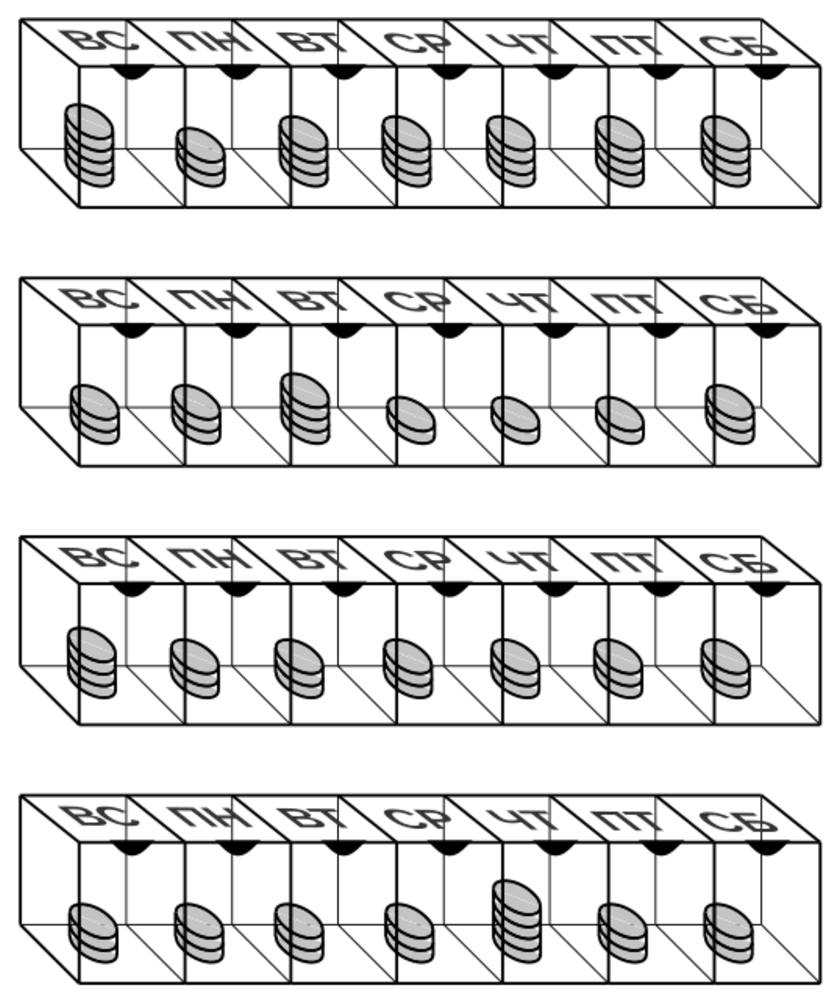
\includegraphics[scale=0.5]{Figs/Handicaps/box1-ru}
\end{figure}

Первая ячейка справа от кучи, содержащая $k-1$ таблеток, будет той, из которой нужно взять таблетку.
Если ячейки с $k-1$ таблетками нет, тогда нужно взять таблетку из кучи.
В почти всех случаях надпись на ячейке, из которой берётся таблетка, правильная, то есть совпадает с текущим днём недели.

Таким образом, например, коробочки на рисунке выше подготовлены для приёма таблетки во вторник, субботу, понедельник и четверг, соответственно.

Исключением является момент, когда у профессора остаётся одна последняя таблетка.
В предыдущий день он обнаружил две оставшиеся таблетки вместе в ячейке, помеченной соответствующим днём недели, и он одну оттуда взял (согласно правилу, что если нет ячейки размером на один меньше, чем куча, надо брать из кучи).
Теперь последняя таблетка лежит в ячейке, помеченной \emph{вчерашним} днём, и эту таблетку он принимает сегодня.

Легко заметить, что если таблетки разложены должным образом, тогда их конфигурация сохраняет верность правилам до последней таблетки.
Но всегда ли возможно правильно настроить эту схему, когда приходят новые таблетки? Да, действительно, существует единственная правильная конфигурация для любого данного числа таблеток и любого данного утра дня недели.
И эта та конфигурация, которую профессор создаёт, когда получает таблетки.
Профессор просто вычисляет день, когда должна быть принята последняя таблетка (а именно, вчерашний день недели плюс число таблеток по модулю 7,
предполагается, что сегодняшнюю таблетку он ещё не выпил).
Конечно, дни недели пронумерованы последовательно  по модулю 7, но не имеет значения, который день номер~1.

Если, скажем, в среду утром пришло 32 таблетки, то профессор знает, что последнюю таблетку надо будет принять в субботу (из ячейки \textsc{пт}!) Из этого следует, что ячейка \textsc{пт} содержит кучу.
Профессор кладёт шесть таблеток в \textsc{пт}, по четыре таблетки в \textsc{сб}, \textsc{вс}, \textsc{пн}, \textsc{вт}, и по пять в \textsc{ср} и \textsc{чт}.
И теперь у него всё устроено должным образом, чтобы принять таблетку для среды.
\heart

Было бы уместно задать вопрос:
«А что, если у нас меньше, чем семь ячеек?
При каком наименьшем числе ячеек наша задача имеет решение?
А что, если в неделе $d$ дней, вместо семи,
каково тогда наименьшее возможное число ячеек, как функция от $d$?»

Отметим, что профессорское решение работает и на Юпитере, где в неделе $d$ дней ($d>1$), и где коробочки для таблеток, конечно же, имеют $d$ ячеек.
В случае $d=2$ это сводится к тому, что в одной ячейке держится на одну или две таблетки больше.
Решение для двух ячеек может быть использовано для любого чётного , так как человек, принимающий таблетки, знает, какой сейчас день этой чётной недели, и знает чётность этого дня.
Так что наличие двух ячеек достаточно и, конечно, необходимо, когда $d$ чётно.

Однако, две ячейки не сработают, если $d$ нечётно.
Там непременно присутствуют два последовательных дня недели, которые должны будут сойтись к одинаковой одно-таблеточной конфигурации, так что, когда человек видит такую конфигурацию в первый из этих дней, он не может сказать, принял ли он таблетку в этот день или нет.

Читателю, прошедшему уже такой долгий путь, не составит труда убедить себя, что при нечётных достаточно трёх ячеек.
Но придумать простой алгоритм с тремя ячейками для семидневной недели довольно сложно.
Следующая схема мнемонически использует двоичную запись.

Пронумеруем дни недели, начиная с воскресенья = 1 и заканчивая субботой = 7, числами по модулю 7.
Схема включает в себя семь «типов конфигураций», пронумерованных от 1 до 7, а конфигурации в каждом типе определяются по бинарному представлению номера типа.
При этом мы считаем, что ячейки располагаются в линейном порядке («левая», «центральная» и «правая») то есть нам не будет нужен циклический порядок.

Так, например, тип $1=001_2$ требует, чтобы правая ячейка была задействована как куча с гораздо большим количеством таблеток, чем будет в каждой из двух остальных.
Тип $3 = 011_2$ требует, чтобы в левой ячейке было существенно меньше таблеток, чем в любой из двух остальных ячеек, а тип 7$ = 111_2$ --- чтобы заполненность ячеек держалась почти на одном уровне.

Точнее, типы 1, 2 и 4 имеют кучи (справа, в центре и слева, соответственно), в которых на две или три таблетки больше, чем в любой из двух других ячеек.
При этом эти две другие ячейки, если они различны, то упорядочены так, что б\'{о}льшая ячейка находится правее.

Типы 3, 5 и 6 имеют oсобую наименьшую ячейку слева, в центре или справа, соответственно.
Две другие ячейки содержат каждая на две таблетки больше, если они одинаковые.
Если нет, то они различаются по размеру не больше, чем на одну таблетку, и б\'{о}льшая ячейка расположена правее и содержит на 2 или 3 таблетки больше, чем самая маленькая.

Тип 7 требует, чтобы содержимое ячеек отличалось друг от друга максимум на одну таблетку, с меньшими ячейками справа (см. таблицу).

Стратегия теперь следующая: если в день $D$ получено $P$ таблеток, то они распределяются согласно типу $P+D \pmod 7$.
Таблетки берутся так, чтобы сохранялся тип.

В частности, каждый день, профессор, смотрит на тип $T$ и поступает следующим образом:
если в день $D$ он видит $P>3$ таблеток и $D+P\ne T\pmod 7$, значит, он уже в этот день таблетку принял.
В противном случае, он берёт таблетку из особой ячейки, в результате оставляя конфигурацию того же типа.

\begin{center}
  \begin{tabular}{ l | c  c c c }
     & 3 таб. & 4 таб & 5 таб & 6 таб \\ \hline
    тип 1 & 003 & 013 & 113 & 114 \\ 
    тип 2 & 030 & 031 & 131 & 141 \\ 
    тип 3 & 012 & 022 & 023 & 123\\ 
    тип 4 & 300 & 301 & 311 & 411\\ 
    тип 5 & 102 & 202 & 203 & 213\\ 
    тип 6 & 120 & 220 & 230 & 231\\ 
    тип 7 & 111 & 211 & 221 & 222
  \end{tabular}
\end{center}

Когда остаётся три или меньше таблетки, становится трудно следовать какому-либо типу, но можно воспользоваться правилом «слева-направо» для типов, чтобы решать, как необходимо менять дальше конфигурации.
Это сводится к использованию следующей таблицы:

\begin{figure}[h!]
\centering
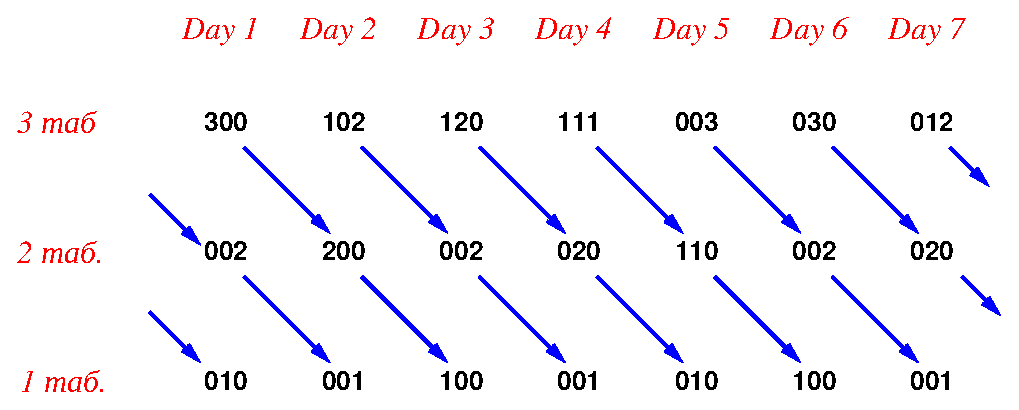
\includegraphics[scale=0.6]{Figs/Handicaps/3box-ru}
\end{figure}

Чтобы воспользоваться таблицей, нужно найти в ней запись, соответствующую $D$ и $P$;
если такая имеется, то нужно взять таблетку так, чтобы после получилась конфигурация ниже и направо (следуя по диагонали).
В противном случае, конфигурация будет соответствовать дню $D+1$, и, значит, таблетка за этот день уже принята.
